\clearpage

\section{Modelltheorie}

Nachdem in den letzten Teilen wichtige Konzepte der Mengenlehre und die Gödelschen Unvollständigkeitssätze vermittelt wurden, sollen werden hier nun zentrale Ideen der Modelltheorie gezeigt.

\subsection{Erhaltungssätze (Charakterisierungssätze)}

Ein wichtiges Ziel der Modelltheorie ist es, einen Zusammenhang zwischen Syntax und Semantik zu bilden. Allgemein lässt sich dies formalisieren: Eine Formel $\psi\in FO$ hat eine semantische Eigenschaft $P$ gdw. wenn $\psi$ äquivalent zu einer Formel in einem Fragment $F_p\subseteq FO$ ist.

Beispiele dafür sind der Satz von \textit{\L os-Tarski} und \textit{Satz von Benthem}.

\paragraph{Satz von \L o\'{s}-Tarski}
$\psi\in FO$ ist erhaltend unter Substrukturen (d.h. wenn $\mathfrak{B}\models \psi$ und $\mathfrak{A}\subseteq\mathfrak{B}$, dann ist auch $\mathfrak{A}\models\psi$) gdw. $\psi$ äquivalent ist zu einer universellen Formel $\forall \bar{x}(\varphi)$, wobei $\varphi$ quantorenfrei ist.

\paragraph{Satz von van Benthem}
$\psi(x)\in FO$ ist invariant unter Bisimulation (d.h. wenn $\K\models \psi(v)$ und $\K,v\sim \K',v'$, dann gilt auch $\K'\models \psi(v')$) gdw. $\psi(x)$ äquivalent zu einer Formel $\psi'\in ML$ ist.

In beiden Fällen gilt, dass die Richtung von Syntax zur Semantik trivial ist. Beispielsweise ist die Bisimulations-Invarianz von zu einer Modallogischen Formel äquivalenten $FO$-Formel klar. Die Rückrichtung ist aber alles andere als offensichtlich und werden daher noch genauer in diesem Kapitel betrachtet.

\subsection*{Refresher zur Modallogik}

Für eine Formel $\psi$ gilt $\psi\in ML$ (Modallogik), wenn $\psi$ induktiv definiert ist, als
\[\psi\coloneqq P_i \,\vert\, \neg\psi \,\vert\, \psi\land\psi \,\vert\, \psi\lor\psi \,\vert\, \psi\rightarrow\psi \,\vert\, \lozenge\psi \,\vert\, \square\psi.\]

Modell einer Modallogischen Formel ist eine Kripkestruktur $\K=(V,(P_i)_{i\in I}, E)$. Wobei $V$ eine Menge an Knoten, $E$ eine zweistellige Kantenrelation und $P_i$ für jedes $i\in I$ eine einstellige Relation ist, welche die Eigenschaften von Knoten darstellt.
\\
\\
Semantisch ist $ML$ definiert als
\begin{itemize}
	\item $\K,v\models P_i$ gdw. $v\in P_i$.
	\item Die Junktoren $\land,\lor,\rightarrow$ sind wie aus $AL$ oder $FO$ bekannt.
	\item $\K,v\models \lozenge \psi$ genau dann, wenn es ein $w\in vE=\{w:(v,w)\in E\}$ gibt, mit $\K,w\models \psi$.
	\item $\K,v\models \square \psi$ genau dann, wenn für alle $w\in vE$ gibt, mit $\K,w\models \psi$.
\end{itemize}
Die Modallogik lässt sich in die Prädikatenlogik einbetten. Es gibt also eine Abbildung mit $\psi\mapsto \psi^\ast(x)$, bzw. nach Formelaufbau:

\begin{itemize}
	\item $P_i\mapsto P_i x$
	\item $\psi_1\circ \psi_2\mapsto \psi_1^\ast(x)\circ\psi_2^\ast(x)$ für $\circ\in\{\land,\lor,\rightarrow\}$
	\item $\lozenge\psi\mapsto\exists y (Exy \land \psi^\ast(y))$
	\item $\square\psi \mapsto \forall y (Exy\rightarrow \psi^\ast(y))$
\end{itemize}
Das Bild dieser Abbildung wird als modales Fragment der Prädikatenlogik bezeichnet.
\\
\\
Eine Bisimulation zwischen zwei Transitionssystemen $\K=(V,(P_i)_{i\in I}, E)$ und $\K'=(V',(P_i')_{i\in I}, E')$ ist eine Relation $Z\subseteq V\times V'$ so, dass für alle $(v,v')\in Z$ gilt:
\begin{itemize}
	\item $v\in P_i\Leftrightarrow v'\in P_i'$
	\item Hin: Zu jedem Knoten $w\in vE$ existiert ein $w'\in v'E'$ so, dass $(w,w')\in Z$.
	\item Her: Zu jedem Knoten $w'\in v'E'$ existiert ein $w\in vE$ so, dass $(w,w')\in Z$,
\end{itemize}
Es lässt sich erkennen, dass $ML$ Bisimulationsinvariant ist. Das heißt, wenn $\K,v\models \psi$ und $\K,v\sim \mathfrak{K'},v'$, dann ist auch $\K',v'\models \psi$.


\subsection*{Weiter mit Erhaltungssätzen}

\begin{definition}[Existenziell-positiv]
	Eine $FO$-Formel ist \textit{existenziell positiv} ($\Sigma_1^+$-Formel), wenn sie weder Allquantoren, noch Negationen oder Implikationen enthält, also aus Atomen mit $\land$, $\lor$ und $\exists$ aufgebaut ist.
\end{definition}

\begin{definition}[Existenzielle und universelle Formeln]
	Eine $FO$-Formel ist existenziell ($\Sigma$-Formel), wenn sie die Form $\exists \bar{x} \varphi$ mit quantorenfreiem $\varphi$ hat.
	
	Eine $FO$-Formel ist universell ($\Pi_1$-Formel), wenn sie die Form $\forall \bar{x} \varphi$ mit quantorenfreiem $\varphi$ hat.
\end{definition}
Induktiv ist weiter definiert, dass eine Formel $\psi$ eine $\Sigma_{n+1}$-Formel ist, wenn $\psi=\exists\bar{x}\varphi$ gilt und $\varphi$ eine $\Pi_n$-Formel ist. Dual ist dies für $\Pi_{n+1}$-Formeln definiert. Eine $\Pi_{n+1}$-Formel ist von der Form $\forall \bar{x}\varphi$ für ein $\varphi$, welches eine $\Sigma_n$-Formel ist. Offensichtlich sind diese Formeln in Pränex-Normalform. Auch lässt sich erkennen, dass wenn $\varphi$ eine $\Sigma_n$-Formel ist, $\neg\varphi$ eine $\Pi_n$-Formel wird.

\begin{definition}[Abgeschlossenheit]
	Eine Formel $\psi(x)$ ist abgeschlossen unter einer Abbildung $f:\mathfrak{A}\to\mathfrak{B}$, wenn für alle $\bar{a}$ aus $\mathfrak{A}$ gilt $\mathfrak{A}\models\psi(\bar{x})\Rightarrow\mathfrak{B}\models\psi(f\bar{a})$.
\end{definition}

Ein \textit{Homomorphismus} $h$ ist eine Abbildung von $\mathfrak{A}$ nach $\mathfrak{B}$, für welche gilt, wenn $\bar{a}\in R^\mathfrak{A}$, dann ist $(h \bar{a})\in R^\mathfrak{B}$ für ein Relationssymbol $R$ und analog für Funktionen.

Verglichen dazu ist ein \textit{starker Homomorphismus} ein \textbf{injektiver} Homomorphismus $h$, für den gilt $\bar{a}\in R^\mathfrak{A}$ \textbf{gdw.} $(h \bar{a})\in R^\mathfrak{B}$. Einen starken Homomorphismus nennt man auch eine \textit{Einbettung}.

\begin{lemma}
	Jede $\Sigma^+_1$-Formel bleibt unter Homomorphismen erhalten.
	\label{Sigma1UnterHom}
\end{lemma}
\begin{proof}
	Sei $h:\mathfrak{A}\to\mathfrak{B}$ ein Homomorphismus. Zunächst gilt für jeden Term $t(\bar{x})$:
	\[h(\llbracket t(\bar{a})\rrbracket^\mathfrak{A})=\llbracket t(h\bar{a})\rrbracket^\mathfrak{B}, \tag{$(\ast)$}\]
	denn:
	\begin{itemize}
		\item $t\coloneqq x_i$: klar, da beide Seiten den Wert $ha_i$ \glqq erhalten\grqq{}.
		\item $t\coloneqq gt_1\dots t_k$: Dann ist
		\begin{alignat*}{2}
			h\llbracket t(\bar{a})\rrbracket^\mathfrak{A} 
			&= &&h(g^\mathfrak{A}(\llbracket t_1(\bar{a})\rrbracket^\mathfrak{A},\dots,\llbracket t_k(\bar{a})\rrbracket^\mathfrak{A})) \\
			\overset{h \text{ Hom.}}&{=} &&g^\mathfrak{B}(h\llbracket t_1(\bar{a})\rrbracket^\mathfrak{A},\dots,h\llbracket t_k(\bar{a})\rrbracket^\mathfrak{A}) \\
			\overset{\text{IV.}}&{=} &&g^\mathfrak{B}(\llbracket t_1(h\bar{a})\rrbracket^\mathfrak{B},\dots,\llbracket t_k(h\bar{a})\rrbracket^\mathfrak{B}) \\
			&= &&\llbracket t(h\bar{a})\rrbracket^\mathfrak{B}.
		\end{alignat*}
	\end{itemize}
	Durch eine Induktion über den Formelaufbau lässt sich dann diese Eigenschaft auch für Formeln $\psi$ feststellen:
	\begin{itemize}
		\item $\psi\coloneqq t_1(\bar{x})=t_2(\bar{x})$:
		\begin{alignat*}{2}
			\mathfrak{A}\models t_1(\bar{a})=t_2(\bar{a})
			&\Longleftrightarrow &&\llbracket t_1(\bar{a})\rrbracket^\mathfrak{A} = \llbracket t_2(\bar{a})\rrbracket^\mathfrak{A} \\
			&\Longrightarrow &&h\llbracket t_1(\bar{a})\rrbracket^\mathfrak{A} = h\llbracket t_2(\bar{a})\rrbracket^\mathfrak{A} \tag{$\vartriangle$}\\
			\overset{(\ast)}&{\Longleftrightarrow} &&\llbracket t_1(h\bar{a})\rrbracket^\mathfrak{B} = \llbracket t_2(h\bar{a})\rrbracket^\mathfrak{B} \Leftrightarrow \mathfrak{B}\models t_1(h\bar{a})=t_2(h\bar{a}).
		\end{alignat*}
		
		\item $\psi\coloneqq R t_1(\bar{x}),\dots,t_k(\bar{x})$:
		\begin{alignat*}{2}
			\mathfrak{A}\models R t_1(\bar{a}),\dots,t_k(\bar{a})
			&\Longleftrightarrow &&(\llbracket t_1(\bar{a})\rrbracket^\mathfrak{A},\dots,\llbracket t_k(\bar{a})\rrbracket^\mathfrak{A})\in R^\mathfrak{A} \\
			\overset{h\text{ Hom.}}&{\Longrightarrow} &&(h\llbracket t_1(\bar{a})\rrbracket^\mathfrak{A},\dots,h\llbracket t_k(\bar{a})\rrbracket^\mathfrak{A})\in R^\mathfrak{B} \tag{$\bigcirc$} \\
			\overset{(\ast)}&{\Longleftrightarrow} &&(\llbracket t_1(h\bar{a})\rrbracket^\mathfrak{B},\dots,\llbracket t_k(h\bar{a})\rrbracket^\mathfrak{B})\in R^\mathfrak{B} \Leftrightarrow \mathfrak{B}\models R t_1(h\bar{a}),\dots,t_k(h\bar{a}).
		\end{alignat*}
		
		\item Die Fälle $\psi\coloneqq\varphi\land\varphi'$ und $\psi\coloneqq \varphi\lor \varphi'$ sind klar.
		
		\item $\psi\coloneqq \exists y \varphi(\bar{x},y)$:
		\begin{alignat*}{2}
			&  &&\mathfrak{A}\models \exists y \varphi(\bar{a},y) \\
			&\Longrightarrow &&\text{es ex. } b \text{ mit } \mathfrak{A}\models\varphi(\bar{a},b) \\
			\overset{\text{IV}}&{\Longrightarrow} &&\mathfrak{B}\models \varphi(h\bar{a},hb) \Rightarrow \mathfrak{B}\models \exists y \varphi(h\bar{a},y).
		\end{alignat*}
	\end{itemize}
\end{proof}

\begin{lemma}
	$\Sigma_1$-Formeln $\psi(\bar{x})$ bleiben unter Einbettung erhalten.
\end{lemma}
\begin{proof}
	Sei $h$ eine Einbettung. Ohne Einschränkung lässt sich voraussetzen, dass $\psi(\bar{x})$ in Negations-NF ist. Nun lässt sich die Behauptung durch eine Induktion über den Formelaufbau wie oben zeigen:
	\begin{itemize}
		\item Für $\psi\coloneqq t_1=2t_2$ oder $\psi\coloneqq R t_1,\dots,t_n$ lässt sich dies genauso wie oben zeigen.
		\item Da $h$ injektiv ist, gilt die Folgerung $(\vartriangle)$ auch in die andere Richtung. Man erhält also eine Kette an Äquivalenzen. Dadurch lässt sich diese analog auf den hier beschriebenen Fall $\psi$ anwenden.
		\item Falls $\psi\coloneqq\neg R t_1,\dots,t_n$ lässt sich das Argument wie im vorherigen Beweis verwenden. Die Folgerung von $(\bigcirc)$ wird aber eine Äquivalenz, da $h$ ein starker Homomorphismus ist.
		\item Die Fälle $\psi\coloneqq\varphi\land\varphi'$, $\psi\coloneqq\varphi\lor\varphi'$ und $\exists y \varphi(\bar{x},y)$ lassen sich genauso wie oben beweisen.
	\end{itemize}
\end{proof}

\begin{lemma}
	$\Pi_1$-Formeln bleiben unter Substrukturen erhalten.
	\label{Pi1UnterSubstruk}
\end{lemma}
\begin{proof}
	Seien $\A,\B$ zwei Strukturen mit $\A\subseteq\B$ und $\psi(\bar{x})$ eine $\Pi_1$-Formel. Angenommen, es gilt $\A\models\neg\psi(\bar{a})$ und $\B\models\psi(\bar{a})$ für $\bar{a}$ aus $A$. Dann ist $\neg\psi(\bar{x})$ aber äquivalent zu einer $\Sigma_1$-Formel. Mit Lemma \ref{Sigma1UnterHom} folgt aber $\A\models\neg\psi(\bar{x})\Rightarrow\B\models\neg\psi(\bar{a})$. Widerspruch!
\end{proof}

\begin{definition}
	Eine Folge $(\A)_{i<\alpha}$ von $\tau$-Strukturen ist eine \textit{Kette}, wenn jeweils $\A_i\subseteq\A_j$ für $i<j$. Die Vereinigung $\bigcup_{i<\alpha}\A_i$ einer solchen Kette ist die Struktur $\A$ mit Universum $A=\bigcup_{i<\alpha}A_i$ und
	\begin{itemize}
		\item $\bar{a}\in R^\A$ gdw. $\bar{a}\in R^{\A_i}$ für ein $i<\alpha$ (und daher für alle $j<\alpha$ mit $\bar{a}\in A_j$).
		\item $f^\A(\bar{a})=b$ gdw. $f^{\A_i}\bar{a}=b$ für ein (und dadurch alle) $i<\alpha$ mit $\bar{a}\in A_i$.
	\end{itemize}
\end{definition}
$\varphi(x)$ bleibt Erhalten unter Vereinigung von Ketten, wenn für jede Kette $(\A_i)_{i<\alpha}$ mit $\bar{a}\in A_0$ und $\A_i\models\varphi(\bar{a})$ für alle $i$, dann auch $\bigcup_{i<\alpha}\A_i \models \varphi(\bar{a})$ gilt.

Dies sind nicht alle Formeln. Sei bspw. $\A_i=(\{0,\dots,i\},a^{\N})$. Jedes $\A_i$ hat ein maximales Element, aber $\bigcup\A_i=(\N,<)$ nicht. Das heißt, es gibt $\Sigma_2$-Formeln, welche nicht unter Vereinigung von Ketten erhalten bleiben ($\exists x \forall y (y\leq x)$).

\begin{lemma}
	$\Pi_2$-Formeln bleiben erhalten unter Vereinigung von Ketten.
\end{lemma}
\begin{proof}
	Sei $(\A_i)_{i<\alpha}$ eine Kette, $\A\coloneqq\bigcup_{i<\alpha}\A_i$ und $\bar{a}\subseteq A_0$. Weiter sei $\forall \bar{y} \varphi(\bar{x},\bar{y})$ eine $\Pi_2$-Formel (also $\varphi(\bar{x},\bar{y})$ eine $\Sigma_1$-Formel) so, dass $\A_i\models\forall \bar{y} \varphi(\bar{a},\bar{y})$ für alle $i<\alpha$.
	
	Nun ist zu zeigen, dass $\A\models\forall \bar{y} \phi(\bar{a},\bar{y})$. Angenommen, es existiert ein $\bar{b}\subseteq\A$ mit $\A\models\neg\varphi(\bar{a},\bar{b})$. Da $\vert\bar{b}\vert$ endlich ist, existiert ein $j<\alpha$ mit $\bar{b}\subseteq A_j$. 
	Da $\neg\varphi$ äquivalent zu einer $\Pi_1$-Formel ist und $\A_j\subseteq\A$, folgt wegen Lemma \ref{Pi1UnterSubstruk}, dass $\A_i\models\neg\varphi(\bar{a},\bar{b})$ im Widerspruch zu $\A_j\models\forall\bar{y}\varphi(\bar{a},\bar{y})$.
\end{proof}

\begin{definition}
	Sei $\A$ eine $\tau$-Struktur und $B\subseteq A$. Dann ist $\A_B$ die Expansion von $\A$ um je eine Konstante für $b$ für jedes Element $b\in B$. Ist $T$ eine vollständige Theorie und $\A\models T$, dann ist $T(B)\coloneqq Th(\A_B)$. Im Fall $B=A$ nenne wir $T(A)\coloneqq Th(\A_A)$ das \textit{elementare Diagramm} von $\A$.
\end{definition}
Im Gegensatz dazu ist das Diagramm $D(\A)$ definiert durch $$D(\A)\coloneqq\{\varphi(\bar{a})\in T(A) : \varphi \text{ atomar oder negiert-atomar}\}$$.

\begin{definition}
	$\A$ ist eine \textit{elementare Substruktur} von $\B$ ($\A\preceq\B$), wenn $\A\subseteq\B$ und für jede Formel $\varphi(\bar{x})\in FO$ und alle $\bar{a}$ aus $A$ gilt: $\A\models\varphi(\bar{a})\Leftrightarrow\B\models\varphi(\bar{a})$.
\end{definition}
Dies soll durch zwei Beispiele genauer beleuchtet werden. 

\begin{itemize}
	\item $\A=(\Q,<),\B=(\R,<)$. Dann lässt sich leicht feststellen, dass $\A\preceq\B$.
	\item $\A=(\N\setminus\{0\},<), \B=(\N,<)$. Es gilt $\A\subseteq\B$ und sogar $\A\cong\B$. Aber trotzdem ist $\A\not\preceq\B$. Sei $\varphi(x)$ in einer Struktur wahr, gdw. $x$ das kleinste Element der Struktur ist. Dann ist $\A\models\varphi(1)$, aber $\B\not\models\varphi(1)$.
\end{itemize}

\begin{satz}[Tarski-Vaught-Test]
	Sei $\A\subseteq\B$. Nun sind äquivalent:
	\begin{enumerate}
		\item $\A\preceq \B$.
		\item Für jede Formel $\varphi(\bar{x},y)$ und alle $\bar{a}$ aus $\A$ gilt: $\B\models \exists y \varphi(\bar{a},y)\Rightarrow \B\models\varphi(\bar{a},a')$ für ein $a'\in A$.
	\end{enumerate}
\end{satz}
\begin{proof}
	\textit{1. $\Rightarrow$ 2.}: Sei $\A\preceq\B$ und $\B\models\exists y \varphi(\bar{a},y)$. Dann gilt $\A\models\exists y \varphi(\bar{a},y)$, das heißt $\A\models\varphi(\bar{a},a')$ für ein $a'\in A$. Da $\A\preceq\B$, folgt $\B\models\varphi(\bar{a},a')$.
	
	\textit{2. $\Rightarrow$ 1.}: Das Kriterium des Tests sei erfüllt. Nun ist zu zeigen, dass für jede Formel $\psi(\bar{x})$ und $\bar{a}$ aus $\A$ gilt: $\A\models\psi(\bar{a})\Leftrightarrow \B\models\psi(\bar{a})$. Dies soll wieder durch eine Induktion über den Formelaufbau passieren.
	
	\begin{itemize}
		\item Die atomaren Fälle $\psi\coloneqq x=y$ und $\psi\coloneqq R\bar{x}$, als auch die einfachen Induktionsschritte $\psi\coloneqq \neg\varphi$, $\psi\coloneqq\varphi\land\varphi'$ und $\psi\coloneqq \varphi\lor\varphi'$ sind klar.
		
		\item $\psi\coloneqq\exists y \exists \varphi(\bar{a},y)$:
		\begin{itemize}
			\item $\A\models\exists y\varphi(\bar{a},y)
			\Rightarrow \A\models\varphi(\bar{a},a')\text{ für ein } a'\in A
			\overset{\text{IV}}{\Rightarrow}\B\models\varphi(\bar{a},a')
			\Rightarrow\B\models\exists y \varphi(\bar{a},y)$.
			
			\item $\B\models\exists y\varphi(\bar{a},y)
			\overset{\text{Test}}{\Rightarrow} \B\models\varphi(\bar{a},a')\text{ für ein } a'\in A
			\overset{\text{IV}}{\Rightarrow}\A\models\varphi(\bar{a},a')
			\Rightarrow\A\models\exists y\varphi(\bar{a},y)$.
		\end{itemize}
	\end{itemize}
\end{proof}

\begin{definition}[Elementare Einbettung]
	$f:\A\to\B$ ist eine \textit{elementare Einbettung} ($f:\A\preceq\B$), wenn gilt: $f$ ist eine Einbettung und für alle $\varphi(\bar{x}),\bar{a}$: $\A\models\bar{a}\Leftrightarrow\B\models\varphi(f\bar{a})$. Es ergibt sich dadurch folgendes Verhalten: $\A\cong f[\A]\preceq\B$.
\end{definition}

\begin{definition}[Elementare Kette]
	Eine Kette $(\A_i)_{i\in \alpha}$ ist elementar, wenn $\A_i\preceq\A_j$ für $i\leq j$ gilt.
\end{definition}

\begin{satz}
	Für jede Kette elem. $(\A_i)_{i\in \alpha}$ gilt $\A_k\preceq\bigcup\A_i$ für alle $k<\alpha$.
\end{satz}

\begin{lemma}
	Sei $\A\subseteq\B$ und $\B_A\models Th(\A_A)=T(A)$. Dann ist $\A\preceq\B$.
\end{lemma}
Zur Erinnerung: $T(A)$ ist das elementare Diagramm.
\begin{proof}
	Wenn $\A\models\varphi(\bar{a})$, dann folgt $\varphi(\bar{a})\in T(A)$ und da $\B$ Modell von $T(A)$ ist, gilt $\B\models\varphi(\bar{a})$.
	
	Im Gegensatz ist mit den gleichen Argumenten, sowie der Vollständigkeit von $T(A)$ einsehbar, dass $\A\not\models\varphi(\bar{a}) \Rightarrow \neg\varphi(\bar{a})\in T(A) \Rightarrow \B\not\models\varphi(\bar{a})$ gilt.
\end{proof}


\subsubsection*{Typen}

\begin{definition}
	Sei $\A$ eine $\tau$-Struktur, $B\subseteq A$ und $n\in \N$. Dann ist definiert:
	\begin{enumerate}
		\item Ein \textit{$n$-Typ} von $\A$ über $B$ ist eine Menge $p$ von Formeln $\varphi(x_0,\dots,x_{n-1})\in FO(\tau\cup B)$ so, dass $p\cup Th(\A_B)$ erfüllbar ist.
		\item $tp_\A(\bar{a}/B)\coloneqq \{\varphi(\bar{x}) \in FO(\tau\cup B) : \A_B\models\varphi(\bar{a})\}$.
		\item $\A$ \textit{realisiert} den Typen $p$ über $B$, wenn ein Tupel $\bar{a}$ aus $\A$ existiert mit $p\subseteq tp_\A(\bar{a}/B)$.
		\item Ein Typ $p$ über $B$ ist \textit{vollständig}, wenn kein $n$-Typ $q$ von $\A$ über $B$ existiert, mit $p\subsetneqq q$.
		\item Der \textit{Stone-Raum} $S^n(B)$ ist die Menge der vollständigen $n$-Typen über $B$.
	\end{enumerate}
\end{definition}

Zwei Beispiele sollen dies verdeutlichen. Es sei $\A=(\omega,s,0)$, wobei $s(n)\coloneqq n+1$ die Sukzessor-Funktion ist. Dann ist $S^1(\emptyset)\supseteq\{p_0,p_1,\dots\}\cup\{p_\infty\}$, mit
\begin{itemize}
	\item $p_n\coloneqq tp(n/\emptyset)\models x=\underbrace{ss\cdots s}_{n\text{-mal}}0$ für ein $n\in \N$.
	\item $p_\infty\models\{x\neq\underbrace{ss\cdots s}_{n\text{-mal}}0 : n\in\omega\}$.
\end{itemize}
Es lässt sich feststellen, dass $p_\infty$ nicht in $\A$ realisiert ist. Die Menge $\{x\neq\underbrace{ss\cdots s}_{n\text{-mal}}0 : n\in\omega\}\cup Th(\omega,s,0)$ ist aber dennoch erfüllbar. Dies lässt sich mithilfe des Kompaktheitssatzes zeigen. Offensichtlich ist jede endliche Teilmenge erfüllbar, demnach also also auch die gesamte Menge.
\\
\\
Als zweites Beispiel soll $\A=(\Q,<)$ für ein festes, aber beliebiges $A\subseteq \Q$ betrachtet werden. Nun gibt es für ein festes $a\in A$ folgende Typen:
\begin{itemize}
	\item[$(a)$] $p\models x=a$.
	\item[$(a^+)$] $p\models x>b$ für alle $A\ni b\leq a$ und $p\models x<b$ für alle $A\ni b>a$. Die erste Folgerung besagt, dass $x$ größer als alle $b\in A$ ist, welche kleiner-gleich $a$ sind. Insbesondere ist $x$ also größer als $a$. Die Zweite Formel besagt, dass $x$ kleiner als das nächste $b\in A$ ist, welches größer als $a$ ist. Wenn $a'$ also die nach $a$ nächste Zahl in $A$ ist, ist $x\in(a,a')$. Bzw. \textit{$x$ ist direkt über $a$}.
	\item[$(a^-)$] Dieser Typ besagt, dass \textit{$x$ direkt unter $a$} ist und lässt sich analog zu $(a^+)$ darstellen.
\end{itemize}
Zusätzlich gibt es noch den Typen $(+\infty)$ mit $p\models x>a$ für alle $a\in A$, sowie den dazu analog definierten Typen $(-\infty)$.

Falls $A=A_0\dot{\cup}A_1$ gilt, $A_0$ kein größtes, $A_1$ kein kleinstes Element hat und $a_0<a_1$ für beliebige $a_0\in A_0,a_1\in A_1$ gilt, dann existiert noch der Typ $p$ mit $p\models x>a$ für $a\in A_0$ und $p\models x<a$ für $a\in A_1$.

\begin{lemma}
	Sei $\A$ eine $\tau$-Struktur, $\B\subseteq\A$ und $p$ ein $n$-Typ über $B$. Dann gibt es eine elementare Erweiterung $\C\succeq\A$ in der $p$ realisiert ist.
\end{lemma}
\begin{proof}
	Sei $\Phi\coloneqq p \cup Th(\A_A)$. Wenn $\C\models\Phi$, dann ist $\C\succeq\A$ und es gibt $\bar{c}$ mit $tp_\C(\bar{c}/A)\supseteq p$. Es muss also gezeigt werden, dass $\Phi$ erfüllbar ist. Wegen des Kompaktheitssatzes reicht es zu zeigen, dass jede endliche Teilmenge $\Phi_0\subseteq \Phi$ erfüllbar ist. Sei also $\Phi_0\coloneqq\{\varphi_1,\dots,\varphi_n\}\subseteq\Phi$.
	
	In $\Phi_0$ können nur endlich viele Konstanten aus $B$ und nur endlich viele aus Konstanten aus $A\setminus B$ vorkommen. Es gilt also $\bigwedge\Phi_0=\varphi_1\land\dots\land\varphi_n=\psi(\bar{x},\bar{b})\land\varphi(\bar{b},\bar{c})$ mit $\bar{b}\subseteq B,\bar{c}\subseteq A\setminus B$. 
	Die Formel $\psi(\bar{x},\bar{b})$ entspricht somit den Formeln, die aus $p$ und die Formel $\varphi(\bar{b},\bar{c})$ denen, die aus $Th(\A_A)$ stammen. Es folgt also $\A\models\varphi(\bar{b},\bar{c})$ bzw. $\exists\bar{y}\varphi(\bar{b},\bar{y})\in Th(\A_B)$. 
	Da $p$ ein Typ über $B$ ist, existiert ein Modell $\D$ von $\psi(\bar{x},\bar{b})\land\exists\bar{y}\varphi(\bar{b},\bar{y})$ so, dass also $\D,\bar{e}\models \psi(\bar{e},\bar{b})\land\exists\bar{y}\varphi(\bar{b},\bar{y})$.
	Wähle nun $\bar{d}$ so, dass $\D\models\varphi(\bar{d},\bar{b})$. $\D$ ist dann ein Modell von $\Phi_0$. Nach dem Kompaktheitssatz muss also auch ein Modell von $\Phi$ existieren.
\end{proof}

\begin{satz}[Amalgamationssatz]
	Seien $\B,\C$ $\tau$-Strukturen und $\bar{a}\subseteq B,\bar{c}\subseteq C$ Folgen von Elementen mit $(\B,\bar{a})\equiv(\C,\bar{c})$. Dann gibt es eine elementare Erweiterung $\D\succeq\B$ und eine elementare Einbettung $f:\C\preceq\D$ mit $f(c_i)=a_i$ für alle $i$. 
	Wenn $\langle\bar{a}\rangle_\B$ die von $\bar{a}$ erzeugte Unterstruktur von $\B$ ist, dann gibt es, da $(\B,\bar{a})\equiv(\C,\bar{c})$, eine Einbettung $g:\langle\bar{a}\rangle_\B\to\C$ mit $g(\bar{a})=\bar{c}$. Es ergibt sich ein Zusammenhang wie in Abbildung \ref{AmalgamationssatzAbb}.
	\label{Amalgamationssatz}
\end{satz}

\begin{proof}
	Sei $T\coloneqq Th(\B_B)\cup Th(\C_C)$. Behauptung: $T$ ist erfüllbar. Sei $T_0\subseteq T$ endlich und $\varphi(\bar{a},\bar{c}')$ die Konjunktion der Formeln aus $T_0\cap Th(\C_C)$ mit $\bar{c}'\subseteq C\setminus \bar{a}$.
	
	Wenn $T_0$ nicht erfüllbar wäre, dann würde $Th(\B_B)\models\neg\varphi(\bar{a},\bar{c}')$ gelten. 
	Da die Konstanten $\bar{c}'$ nicht in $B$ vorkommen folgt $Th(\B_B)\models\forall\bar{y}\neg\varphi(\bar{a},\bar{y})$.
	Auf Grund der elementaren Äquivalenz folgt aber aus $\B,\bar{a}\models\forall\bar{y}\neg\varphi(\bar{a},\bar{y})$, dass $\C,\bar{a}\models\forall\bar{y}\neg\varphi(\bar{a},\bar{y})$, was aber im Widerspruch zu $\varphi(\bar{a},\bar{c}')\in Th(\C_C)$ steht. 
	Also ist $T_0$ erfüllbar und nach dem Kompaktheitssatz ist auch $T$ erfüllbar.
	\\
	\\
	Sei $\D^+=(\D, B^{\D^+}\cup C^{\D^+})$ mit $D^+\models T$. Da $(\D,B^{\D^+})\models Th(\B_B)$ kann man annehmen, dass $\D\succeq\B$ und $\bar{b}^{\D^+}=\bar{b}$ für alle $\bar{b}\subseteq B$.
	
	Setze $f(c)=c^{\D^+}$ für alle $c\in C$. Da $(\D,C^{\D^+})\models Th(\C_C)$ ist $f:C\to D$ eine elementare Einbettung. 
	Schließlich ist $f(a)=a^{\D^+}=a$ für alle $a$.
\end{proof}

Daraus ergibt sich auch einige Folgerung: 
\begin{enumerate}
	\item Sei $\B\equiv \C$. Dann existiert ein $\D\succeq\B$ mit elementarer Einbettung $f:\C\preceq\D$.
	\item Wenn $\A\preceq\B$ und $\A\preceq\C$, dann gilt mit dem Amalgamationssatz ein $\D\succeq\B$ mit einer elementaren Einbettung $f:\C\preceq\D$. Setzt man nun $\C'\coloneqq f(\C)$, erhält man einen Zusammenhang wie in Abbildung \ref{AmalgamationssatzKorollar} dargestellt.
\end{enumerate}


\begin{figure}[h]
		\sidesubfloat[]{
			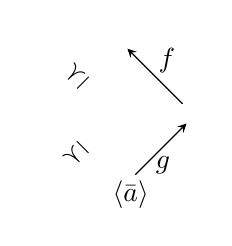
\begin{tikzpicture}
				\draw (0, 1cm) node {$\D$};
				\draw (-1cm, 0) node {$\B$};
				\draw (1cm, 0cm) node {$\C$};
				\draw (0.2cm, -1cm) node {$\langle\bar{a}\rangle_{\B}$};
				
				\path (-1cm, 0) edge [draw=none]
				node [sloped, auto=false,
				allow upside down] {$\preceq$} (0, 1cm);
				
				\draw[-stealth] (0.85cm, 0.15cm) -- (0.15cm, 0.85cm); 
				\draw (0.65cm, 0.7cm) node {$f$};
				
				\path (0, -1cm) edge [draw=none]
				node [sloped, auto=false,
				allow upside down] {$\preceq$} (-1cm, 0);
				
				\draw[-stealth] (0.25cm, -0.75cm) -- (0.9cm, -0.1cm); 
				\draw (0.6, -0.63) node {$g$};
			\end{tikzpicture}
			\label{AmalgamationssatzAbb}
		}
		\hspace{2cm}
		\sidesubfloat[]{
			\begin{tikzpicture}
				\draw (0, 1cm) node {$\D$};
				\draw (-1cm, 0) node {$\B$};
				\draw (1cm, 0cm) node {$\C'$};
				\draw (0cm, -1cm) node {$\A$};
				
				\path (-1cm, 0) edge [draw=none]
				node [sloped, auto=false,
				allow upside down] {$\preceq$} (0, 1cm);
				
				\path (1cm, 0) edge [draw=none]
				node [sloped, auto=false,
				allow upside down] {$\preceq$} (0, 1cm);
				
				\path (0, -1cm) edge [draw=none]
				node [sloped, auto=false,
				allow upside down] {$\preceq$} (-1cm, 0);
				
				\path (0, -1) edge [draw=none]
				node [sloped, auto=false,
				allow upside down] {$\preceq$} (1cm, 0);
			\end{tikzpicture}
			\label{AmalgamationssatzKorollar}
		}
	\caption{Darstellung des Amalgamationssatzes (a) und dessen Folgerung (b)}
\end{figure}

\begin{satz}
	Zu jeder Struktur $\A$ existiert eine elementare Erweiterung $\C$ so, dass Typ $p$ über $A$ in $\C$ realisiert ist.
\end{satz}
\begin{proof}
	Sei $(p_\alpha)_{\alpha<\kappa}$ die Aufzählung aller vollständigen Typen über $A$. Für jedes $\alpha<\kappa$ wählen wir eine elementare Erweiterung $\B_\alpha\succeq\A$ in der $p_\alpha$ realisiert ist.
	Konstruiere eine elementare Kette $(\C_\alpha)_{\alpha<\kappa}$ wie folgt:
	\begin{itemize}
		\item $\C_0\coloneqq\A$.
		\item $\C_\lambda\coloneqq\bigcup_{\alpha<\lambda}C_\alpha$ für Limesordinale $\lambda$.
		\item $\C_{\alpha+1}$ ist eine elementare Erweiterung von $\C_\alpha$ mit der elementaren Einbettung $f:B_\alpha\to\C_{\alpha+1}$ so, dass $f(a)=a$ für $a\in A$.
	\end{itemize}
	Setze $\C\coloneqq\bigcup\limits_{\alpha<\kappa}\C_\alpha(=\C_\kappa)$. $\C$ ist eine elementare Erweiterung aller $C_\alpha$ und damit auch von $\A$ und realisiert jeden Typen über $A$.
\end{proof}

\begin{satz}
	Seien $\B,\C$ $\tau$-Strukturen und $\bar{a}$ ein Tupel aus $B$. Zusätzlich sei $f:\langle\bar{a}\rangle_\B\to\C$ so, dass $\C\models\varphi(f\bar{a})\Rightarrow\B\models\varphi(\bar{a})$ für $\Sigma_1$-Formeln $\varphi(\bar{x})$ gilt. Dann existiert eine elementare Erweiterung $\D\succeq\B$ und eine Einbettung $g:\C\to\D$ mit $gf\bar{a}=\bar{a}$.
\end{satz}
\begin{proof}
	Es lässt sich feststellen, dass $f$ eine Einbettung sein muss. Da $\C\models fa\neq a'\Rightarrow \B\models a\neq a'$ gilt, muss $f$ injektiv sein und betrachtet man $\C\models\neg Rf\bar{x}\Rightarrow\B\models\neg R\bar{a}$ lässt sich feststellen, dass $f$ eine Einbettung ist.
	
	Man nehme nun eine zu $\C$ isomorphe Struktur $\C'$ so, dass $f=\text{id}_{\langle\bar{a}\rangle_\B}$ und $B\cap C'=\langle\bar{a}\rangle_\B$ ist. Sei $T=Th(\B_B)\cup D(\C')$. Zur Erinnerung: $D(C')$ ist das atomare Diagramm von $C'$, also die Menge aller atomaren und negiert-atomaren Formeln, die in $C'$ erfüllt sind. 
	Um zu zeigen, dass $T$ erfüllbar ist, soll wieder der Kompaktheitssatz verwendet werden. 
	Sei $T_0\subseteq T$ also endlich und $\varphi(\bar{a},\bar{c}')$ die Konjunktion der endlich vielen atomaren bzw. negiert-atomaren Formeln aus $T_0\cap D(\C')$ mit $c'\subseteq C'\setminus A$.
	
	Wenn $T_0$ unerfüllbar wäre, dann würde $Th(\B_B)\models\neg\varphi(\bar{a},\bar{c}')$ gelten. Also $Th(\B_B\models\forall\bar{y}\neg\varphi(\bar{a},\bar{y})$. Daraus folgt $\B,\bar{a}\models\neg\exists\bar{y}\varphi(\bar{a},\bar{y})$ und mit der von $f$ geforderten Eigenschaft $\C',\bar{a}\models\neg\exists\bar{y}\varphi(\bar{a},\bar{y})$. Dies ist aber ein Widerspruch zu $\varphi(\bar{a},\bar{c})\in D(\C')$.
	
	Der Rest des Beweises verläuft völlig analog zum Beweis des Amalgamationssatzes.
 \end{proof}
 
 Aus diesem Satz lässt sich folgern, dass für zwei $\tau$-Strukturen $\B$ und $\C$, welche die Eigenschaft erfüllen, dass für beliebige $\Sigma_1$-Sätze $\varphi$ gilt $\C\models\varphi\Rightarrow\B\models\varphi$, sich $\C$ in eine elementare Erweiterung von $\B$ einbetten lässt.

\begin{definition}
	Für $\Phi$ sei $\Phi_\forall\coloneqq\{\varphi\in\Pi_1 : \Phi\models\varphi\}$ und $\Phi_\exists\coloneqq\{\varphi\in\Sigma_1 : \Phi\models\varphi\}$.
\end{definition}

\begin{satz}
	Sei $T\subseteq FO(\tau)$ eine Theorie. Dann gilt $\A\models T_\forall$ gdw. eine Erweiterung $\B\supseteq\A$ existiert, mit $\B\models T$.
	\label{ErweiterungErülltTheorie}
\end{satz}
\begin{proof}
	$\Leftarrow$: $\B\supseteq\A$ mit $\B\models T$ impliziert $\B\models T_\forall$ und da $\Pi_1$-Formeln unter Substrukturen sind und $\B\supseteq\A$, folgt $\A\models T_\forall$.
	
	$\Rightarrow$: Es gelte $\A\models T_\forall$. Behauptung: es gibt ein Modell $\C$ von $Th(\A)_\exists\cup T$. Wenn nicht, dann gibt es eine endliche Teilmenge $\{\varphi_0,\dots,\varphi_{n-1}\}\subseteq Th(\A)_\exists$, welche zusammen mit $T$ unerfüllbar sind. D.h. $T\models \neg\varphi_0\land\dots\land\varphi_{n-1}\eqqcolon\psi\in\Pi_1$. Da also $\psi\in T_\forall$ folgt $\A\models\psi$. Dies steht aber im Widerspruch zu $\A\models\{\varphi_0,\dots,\varphi_{n-1}\}$. Es existiert also solch ein Modell $\C$.
	
	Für jeden $\Sigma_1$-Satz $\varphi$ gilt: $\A\models\varphi\Rightarrow\C\models\varphi$. Also kann man $\A$ eine elementare Erweiterung von $\C$ einbetten. Es gibt also eine Einbettung $f$ so, dass $f(\A)\subseteq\D$ und $\D\succeq\C$ gilt. Es gilt $D\models T$. Also existiert ein $\B\supseteq\A$ mit $\B\models T$.
\end{proof}

\begin{satz}[\L o\'{s}-Tarski]
	Sei $T\subseteq FO(\tau)$ eine Theorie und $\Phi\subseteq FO(\tau)$ eine Satzmenge.
	Dann sind äquivalent:
	\begin{enumerate}
		\item Wenn $\A,\B\models T,\A\subseteq\B$ und $\B\models\Phi$, dann auch $\A\models\Phi$ ($\Phi$ bleibt $\mod T$ unter Substrukturen erhalten).
		\item Es gibt eine Satzmenge $\Psi\subseteq\Pi_1$, die nur aus $\Pi_1$-Sätzen besteht so, dass für jedes Modell von $T$ gilt: $\A\models\Phi\Leftrightarrow\A\models\Psi$ (Auf Modellen von $T$ ist $\Phi$ äquivalent zu einer Menge von universellen Sätzen).
	\end{enumerate}
\end{satz}
\begin{proof}
	\textit{2. $\Rightarrow$ 1.}: Diese Richtung lässt sich leicht mithilfe von Lemma \ref{Pi1UnterSubstruk} einsehen.
	
	\textit{1. $\Rightarrow$ 2.}: Setze $\Psi\coloneqq(T\cup\Phi)_\forall$ und sei $\A\models T$.
	Nun gilt $\A\models\Psi \overset{\text{Satz }\ref{ErweiterungErülltTheorie}}{\Longleftrightarrow}$ es ex. $\B\supseteq\A$ mit $\B\models T\cup \Phi \Rightarrow\A\models\Phi$. Also wenn $\A\models\Phi$ dann auch $\A\models\Psi$.
\end{proof}

Daraus lässt sich die in der Einleitung bereits geschilderte Aussage des Satzes folgern: $\varphi(\bar{x})\in FO(\tau)$ bleibt unter Substrukturen erhalten gdw. $\varphi(\bar)$ äquivalent zu einer Formel $\psi(\bar{x})\in\Pi_1$ ist.
\begin{proof}
	Sei $\bar{c}$ ein Tupel von neuen Konstanten. Betrachte die Theorie $T\coloneqq\{\eta \in FO(\tau\cup\{\bar{c}\}) : \models\eta\}$ aller Tautologien über der Signatur $\tau\cup\{\bar{c}\}$. Wähle $\Phi=\{\varphi(\bar{c})\}$. 
	Aus dem Satz von \L o\'{s}-Tarski folgt, dass $\varphi(\bar{c})$ äquivalent zu einer einer Menge von $\Psi$ von universellen Sätzen ist, also $\Psi\models\varphi(\bar{c})$.
	Nach dem Kompaktheitssatz existiert eine endliche Teilmenge $\Psi_0\subseteq\Psi$ so, dass $\Psi_0\models\varphi(\bar{c})$. Setze $\psi(\bar{c})\coloneqq\bigwedge\Psi_0$. Nun ist $\psi(\bar{c})\equiv\varphi(\bar{c})$, also $\psi(\bar{x})\equiv\varphi(\bar{x})$.
\end{proof}

\begin{definition}[$\kappa$-Saturiertheit]
	Eine Struktur $\A$ ist \textit{$\kappa$-saturiert}, wenn jeder Typ von $\A$ über $B$ mit $\vert B \vert<\kappa$ in $\A$ realisiert ist.
\end{definition}

\begin{satz}
	Jede Struktur $\A$ besitzt eine $\omega$-saturierte elementare Erweiterung $\B\succeq\A$.
\end{satz}
\begin{proof}
	Wir definieren wieder eine Folge $(\B_\alpha)_{\alpha<\omega}$ mit
	\begin{itemize}
		\item $\B_0\coloneqq\A$.
		\item $\B_{\alpha+1}\succeq\B_\alpha$ so, dass in $\B_{\alpha+1}$ jeder Typ von $\B_\alpha$ über eine endlichen Konstantenmenge realisiert ist.
	\end{itemize}
	Nun sei $\B\coloneqq\bigcup_{\alpha<\omega}\B_\alpha$. Weiter sei $p$ ein Typ in $\B$ über einer endlichen Konstantenmenge $C\subseteq B$. Dann ist $C\subseteq B_\alpha$ für ein endliches $\alpha$. Nach Konstruktion ist $p$ dann in $\B_{\alpha+1}$ und damit auch $\B$ realisiert.
\end{proof}

\begin{definition}[Modales Fragment]
	Wir definieren die Abbildung $f:ML\to FO$, welche $ML$-Formeln, in $FO$-Formeln übersetzt. Diese ist induktiv definiert als:
	\begin{itemize}
		\item $f(P_i)\coloneqq P_i x$
		\item $f(\psi_1\circ \psi_2)\coloneqq \psi_1^\ast(x)\circ\psi_2^\ast(x)$ für $\circ\in\{\land,\lor,\rightarrow\}$
		\item $f(\lozenge\psi)\coloneqq\exists y (Exy \land \psi^\ast(y))$
		\item $f(\square\psi) \coloneqq \forall y (Exy\rightarrow \psi^\ast(y))$
	\end{itemize}
	Das \textit{Modale Fragment der Prädikatenlogik} $MF\subseteq FO$ ist definiert als $MF\coloneqq\{\psi^\ast(x) : \exists \psi\in ML (f(\psi)=\psi^\ast(x)) \}$.
\end{definition}

\begin{satz}[van Benthem]
	Es sei $\tau=\{P_i:i\in I\}\cup\{E_a : a\in A\}$, wobei für alle $i\in I$, $P_i$ ein einstelliges und für alle $a\in A$, $E_a$ ein zweistelliges Relationssymbol ist.
	
	Eine Formel $\psi(x)\in FO(\tau)$ ist invariant unter Bisimulation (also wenn $\K\models\psi(v)$ und $\K,v\sim\K',v'$, dann auch $\K'\models\psi(v')$) gdw. $\psi(x)$ äquivalent ist, zu einer Formel $\varphi\in ML$.
\end{satz}
\begin{proof}
	$\Leftarrow$: Diese Richtung wurde bereits in MaLo 1 bewiesen.
	
	$\Rightarrow$: Sei $\psi(x)$ invariant unter Bisimulation und $\Phi\coloneqq\{\varphi(x) \in MF(\tau) : \psi(x)\models\varphi(x)\}$ die Menge der modalen Folgerungen aus $\psi(x)$.
	Wir behaupten nun $\Phi\models \psi(x)$. Sobald wir dies gezeigt haben, folgt der Satz von van Benthem. Denn dann gibt es ein endliches $\Phi_0\subseteq\Phi$ so, dass $\Phi_0\models \psi(x)$. Setzt man dann $\varphi^\ast(x)\coloneqq\bigwedge\Phi_0$ ist $\varphi^\ast$ die Übersetzung einer modalen Formel $\varphi$. $\varphi$ ist äquivalent zu $\psi(x)$.
	\\
	\\
	Sei also $\K_0\models\Phi(v_0)$. Zu zeigen ist, dass $K_0\models\psi(v_0)$. Wir definieren $\Theta\coloneqq\{\psi(x)\}\cup Th_{MF}(\K_0,v_0)$, wobei $Th_{MF}(\K_0,v_0)\coloneqq\{\varphi^\ast(x)\in MF : \K_0\models\varphi^\ast(v_0)\}$ ist.
	
	$\Theta$ ist erfüllbar. Ansonsten existieren $\theta_0(x),\dots,\theta_{n-1}(x)\in Th_{MF}(\K_0,v_0)$ so, dass $\psi(x)\cup\{\theta_0(x),\dots,\theta_{n-1}(x)\}$ unerfüllbar ist. 
	Also ist $\psi(x)\models\neg(\theta_0(x)\land\dots\land\theta_{n-1}(x))$ und damit $\neg(\theta_0(x)\land\dots\land\theta_{n-1}(x))\in\Phi$. Demnach also $\K_0\models\neg(\theta_0(v_0)\land\dots\land\theta_{n-1}(v_0))$. Dies ist aber ein Widerspruch zu $\theta_0(x),\dots,\theta_{n-1}(x)\in Th_Mf(\K_0,v_0)$.
	
	Es gibt also ein Modell $\K_1,v_1$ von $\Theta$.
	Seien $\K_0^+\succeq\K_0,\K_1^+\succeq\K_1$ $\omega$-saturierte Erweiterungen von $\K_0$ bzw. $\K_1$. Weiter ist $Th_{MF}(\K_0^+,v_0)=Th_{MF}(\K_0,v_0)=Th_{MF}(\K_1,v_1)=Th_{MF}(\K_1^+,v_1)$.
	
	Es ist bekannt, dass $\K_0,v_0\sim \K_1,v_1 \Rightarrow \K_0,v_0\equiv_{ML}\K_1,v_1$ gilt. Die Rückrichtung gilt aber nicht im allgemeinen.
	
	\begin{lemma}
		Seien $\K,\K'$ $\omega$-saturiert, mit $\K,v\equiv_{ML}\K',v'$. Dann ist $\K,v\sim\K',v'$.
	\end{lemma}
	\begin{proof}
		Sei $Z=\{(u,u') : \K,u\equiv_{ML} \K',u'\}$. Behauptung: $Z$ ist eine Bisimulation.
		
		Wenn $(u,u')\in Z$, dann ist $\K,u\models P_i\Leftrightarrow \K',u'\models P_i$, für alle $i\in I$.
		
		Hin-Eigenschaft: Sei $(u,w)\in E_a$. Zu zeigen ist, dass es ein $w'$ gibt, mit $(u',w')\in E_a'$ so, dass $(w,w')\in Z$. Wir definieren $p=\{E_a u' x\}\cup Th_{MF}(\K,w)$. $p$ ist ein Typ von $\K'$ über $\{u'\}$. 
		Wenn dies nicht der Fall wäre, dann würde ein endliches $Phi_0\subseteq Th_{ML}(\K,w)$ existieren so, dass $\K'\not\models E_a u' w' \land \bigwedge \Phi_0(w')$ für alle $w'$, bzw. $\K'\models\underbrace{\forall y (E_a u' y \rightarrow \neg \bigwedge\Phi_0(y))}_{\alpha(u')}$. Da wir aber $\K,u\equiv_{ML} \K',u'$ vorausgesetzt haben, folgt $\K\models \alpha(u)$, was aber im Widerspruch steht zu $\K\models E_a u w \land \bigwedge\Phi_0(w)$.
		
		Also ist $p$ realisiert in $\K'$, das heißt, es gibt ein $w'$ mit $\K'\models p(w')$. Also ist $(u',w')\in E_a$ und $\K,w\equiv_{ML} K',w'$. Das heißt $(w,w')\in Z$.
		
		Die Her-Eigenschaft lässt sich völlig analog zeigen.
		
		$Z$ ist also eine Bisimulation. Es folgt $\K,v \sim \K',v'$.
	\end{proof}
	
	Mit diesem Lemma können wir einsehen, dass $\K_0^+,v_0\sim \K_1^+,v_1$.
	Da $\K_1,v_1\preceq \K_1^+,v_1$ und $\K_1\models\psi(v_1)$ folgt $\K_1^+\models\psi(v_1)$. Wegen er Bisimulationsinvarianz von $\psi(x)$ gilt dann auch $\K_0^+\models\psi(v_0)$ und da $\K_0,v_0\preceq\K_0^+,v_0$ folgt $\K_0\models\psi(v_0)$. Dies war zu zeigen.
\end{proof}

Mit diesem Satz lässt sich einsehen, dass die Modallogik $ML$ äquivalent zu dem unter Bisimulation abgeschlossenen Fragment der Prädikatenlogik erster Stufe ist. Im Verlauf des Skriptes wird die weitere Modallogik $L_\eta$ eingeführt werden. 
Nun stellt sich die Frage, ob sich auch für diese eine Logik finden lässt, welches Bisimulationsinvariantes Fragment dieser Modallogik entspricht. 
Mit einem noch komplexeren Beweis als dem Satz von van Benthem lässt sich zeigen, dass genau das für die Monadische Logik zweiter Stufe gilt.

Eine weitere Überlegung die man sich machen kann ist die, ob die beiden diskutierten Erhaltungssätze auch für endliche Strukturen gelten. Es lässt sich zeigen, dass dies für die meisten Sätze nicht gilt. Eine Ausnahme stellt hier der Satz von van Benthem dar. Dieser lässt sich auch für endliche Strukturen benutzen.
Jedoch wird in diesem Fall ein anderer Beweis benötigt, als wir hier verwendet haben. Beispielsweise haben wir mithilfe von $\omega$-saturierten Strukturen argumentiert. Diese sind nach Konstruktion im Allgemeinen nicht endlich
Generell lässt sich auch sagen, dass sehr viel kombinatorischer argumentiert werden muss. Sätze wie den Kompaktsheitssatz kann man beispielsweise nicht anwenden. Über Erhaltungssätze soll nun aber genug gesagt sein.

Weiter soll die infinitäre Logik definiert und die aus MaLo 1 bekannten Ehrenfeucht-Fra\"{i}ss\'{e}-Spiele vollständig hergeleitet werden.




\subsection{Infintäre Logik und Ehrenfeucht-Fra\"{i}ss\'{e}-Spiele}

\begin{definition}
	Sei $\tau$ eine Signatur und $\kappa\in Cn^\infty$. Dann ist die infinitäre Logik $L_{\kappa\omega}[\tau]$ definiert als
	\begin{itemize}
		\item Jede atomare Formel $\varphi\in FO(\tau)$ ist in $L_{\kappa\omega}[\tau]$.
		\item Für $\varphi\in L_{\kappa\omega}[\tau]$ sind $\neg\varphi$, $\exists x \varphi$, $\forall x \varphi\in L_{\kappa\omega}[\tau]$.
		\item $\Phi\subseteq L_{\kappa\omega}[\tau]$ sei eine Formel\textbf{menge} mit $\vert\Phi\vert<\kappa$. Dann sind auch $\bigvee\Phi$ und $\bigwedge \Phi$ Formeln aus $L_{\kappa\omega}[\tau]$.
	\end{itemize}
	Zusammenfassend ist $L_{\infty\omega}[\tau]\coloneqq\bigcup_\kappa L_{\kappa\omega}[\tau]$ definiert.
\end{definition}
Man kann schnell feststellen, dass $L_{\omega\omega}[\tau]=FO(\tau)$ ist.

Um dies besser zu verinnerlichen sollen einige Beispiele erläutert werden:
\begin{itemize}
	\item $\varphi_{fin}\coloneqq\bigvee \{\neg\varphi_{\geq n}: n< \omega\} \in L_{\omega_1\omega}$, mit $\varphi_{\geq n}=\exists x_1\cdots \exists x_n(\bigwedge_{1\leq i < j \leq n}x_i\leq x_j)$. 
	Zuerst soll bemerkt werden, dass in diesem Kontext die Schreibweise $\omega_n$ für $\aleph_n$ verwendet wird. Des weiteren gilt
	$$\mathfrak{A}\models\varphi_{fin} \Leftrightarrow A \text{ endlich}.$$
	
	\item Sei $p$ ein Typ über $B$ mit $\vert B\vert<\kappa$. Dann definieren wir $\varphi(\bar{x})=\bigwedge p$ und es gilt $\A\models \exists \bar{x} \varphi(\bar{x})$, also ist $p$ realisiert in $\A$.
\end{itemize}

\begin{satz}
	Der Kompaktheitssatz gilt nicht für $L_{\kappa\omega}$, wenn $\kappa>\omega$.
\end{satz}
\begin{proof}
	Sei $\varphi_{fin}\in L_{\kappa\omega}$ für $\kappa>\omega$. 
	Dann ist offensichtlich $\Phi=\{\varphi_{fin}\}\cup\{\varphi_{\geq n}:n\in\omega\}$ unerfüllbar, aber jede endliche Teilmenge ist erfüllbar.
\end{proof}

\begin{definition}[Quantorenrang]
	Der aus $FO$ bekannte \textit{Quantorenrang} soll nun auch für die infinitäre Logik $L_{\kappa\omega}$ definiert werden. Für $\psi\in L_{\kappa\omega}$ ist $qr(\psi)\in On$ definiert:
	\begin{itemize}
		\item $\psi$ atomar: $qr(\psi)=0$
		\item $qr(\neg\psi)=qr(\psi)$
		\item $qr(\exists x \psi(x))=qr(\forall x \psi(x))=qr(\psi)+1$
		\item $qr(\bigvee \Phi)=qr(\bigwedge \Phi)\coloneqq \sup\{qr(\varphi):\varphi\in \Phi\}$
	\end{itemize}
\end{definition}

Aich hier sollen wieder Beispiele zum besseren Verständnis angegeben werden:
\begin{itemize}
	\item $qr(\varphi_{fin})=\sup\{qr(\varphi_{\geq n}): n < \omega\}=\omega$.
	\item Sei $\varphi(x)\in L_{\omega_1\omega}(<)$ die Formel, die aussagt, dass $x$ nur endlich viele Vorgänger besitzt. Dann ist $qr(\varphi(x))=\omega$ und $qr(\forall x \varphi(x))=\omega+1$.
\end{itemize}

\begin{definition}[Äquivalenzen]
	Wir schreiben $\A\equiv_\alpha\B$, wenn für alle $\varphi\in L_{\infty\omega}$ mit $qr(\varphi)\leq \alpha$ gilt: $\A\models\varphi \Leftrightarrow \B\models\varphi$.
	
	Analog sei $\A\equiv_\infty\B$, wenn für alle $\varphi\in L_{\infty\omega}$ gilt $\A\models\varphi \Leftrightarrow \B\models\varphi$.
\end{definition}

\begin{definition}[Lokaler Isomorphismus]
	Ein \textit{lokaler Isomorphismus} von $\A$ nach $\B$, für relationale Strukturen $\A$ und $\B$ ist eine Abbildung 
	$p$ mit $Def(p)\subseteq A,Bild(p)\subseteq B$ so, dass $p=\emptyset$ oder
	$p:\A\vert_{Def(p)}\xrightarrow{\sim}\B\vert_{Bild(p)}$. 
	$p$ wird dann auch partieller Isomorphismus genannt.
	
	$Loc(\A,\B)$ beschreibt die Menge aller lokalen Isomorphismen von $\A$ nach $\B$.
\end{definition}

Um lokale Isomorphismen zu notieren werden zwei Notationen verwendet. Seien $\bar{a}=(a_1,a_2,\dots,a_n)$ und $\bar{b}=(b_1,b_2,\dots,b_n)$ so, dass $a_i\in A,b_i\in B$ für $1\leq i \leq n$.
Dann sind $p:\bar{a}\mapsto\bar{b}$ und $p=\{(a_1,b_1),(a_2,b_2),\dots,(a_n,b_n)\}$ zwei Notationen für den Isomorphismus $p$.


\subsubsection*{Spiele}

Nun wollen wir Ehrenfeucht-Fra\"{i}ss\'{e}-Spiele für infinitäre Logiken genauer betrachten.
\begin{definition}[Ehrenfeucht-Fra\"{i}ss\'{e}-Spiele]
	Ein \textit{EF-Spiel} $G_\alpha(\A,\B)$ wird von zwei Spielern gespielt. Dem \textit{Herausforderer (I)} und der \textit{Duplikatorin (II)}. 
	
	Eine \textit{Position} ist ein Tupel $(\beta,\A,\bar{a},\B,\bar{b})$, mit $\beta\leq \alpha$, $\bar{a}\subseteq A$, $\bar{b}\subseteq B$ und $\vert\bar{a}\vert = \vert\bar{b}\vert$.
	Die Startposition ist das Tupel $(\alpha, \A,\langle\rangle,\B,\langle,\rangle)$.
	
	Des weiteren soll nun ein \textit{Zug} von der Position $(\beta,\A,\bar{a},\B,\bar{b})$ aus beschrieben werden: I wählt ein $\gamma < \beta$ und ein $c\in A$ oder $d\in B$. Dann wählt II aus der jeweils anderen Struktur ein $d\in B$ oder $c\in A$. Die neue Position ist dann $(\gamma,\A,\bar{a}c,\B,\bar{b}d)$.
	
	Wird eine Position $(\beta,\A,\bar{a},\B,\bar{b})$ erreicht so, dass $\bar{a}\mapsto\bar{b}\notin Loc(\A,\B)$, dann hat I gewonnen, andernfalls endet das Spiel in einer Position $(0,\A,\bar{a},\B,\bar{b})$ mit $\bar{a}\mapsto\bar{b}\in Loc(\A,\B)$. Dann hat II gewonnen.
\end{definition}

Zur Vereinfachung sagen wir \glqq I/II gewinnt $G_\alpha(\A,\B)$\grqq{} für \glqq I/II hat eine Gewinnstrategie für $G_\alpha(\A,\B)$\grqq{}.

\begin{definition}
	Zusätzlich zu dem Spiel $G_\alpha(\A,\B)$ gibt es das Spiel $G_\infty(\A,\B)$. 
	Dieses verhält sich genauso wie das erstere, bloß wird die erste Komponente der Position weggelassen so, dass Partien unendlich lange dauern können.
	Unendliche Partien sind von II gewonnen.
\end{definition}

\begin{definition}[Hin- und Her-Eigenschaft]
	Sei $I\subseteq Loc(\A,\B)$ und $p\in Loc(\A,\B)$. Dann sagen wir $p$ hat die \textit{Hin- und Her- Eigenschaft (HHE)} bzgl. $I$, wenn gilt:
	\begin{itemize}
		\item Hin: $\forall a\in A \exists b\in B p\cup\{(a,b)\}\in I$
		\item Her: $\forall b\in B\exists a\in A p\cup\{(a,b)\}\in I$
	\end{itemize}
\end{definition}
\begin{definition}[Hin- und Her-System]
	Ein Hin- und Her-System $(I_\alpha(\A,\B))_{\alpha\in On}$ zu $\A$ nach $\B$ besteht aus der Folge von Mengen $I_\alpha(\A,\B)\subseteq Loc(\A,\B)$, welche wie folgt definiert ist:
	\begin{itemize}
		\item $I_0(\A,\B)\coloneqq\{p\in Loc_(\A,\B): p \text{ endlich}\}$
		\item $I_{\alpha+1}\coloneqq\{p\in I_\alpha(\A,\B) : p \text{ hat die HHE bzgl. } I_\alpha(\A,\B)\}$
		\item $I_\delta(\A,\B)\coloneqq \bigcap_{\alpha<\delta}I_\alpha(\A,\B)$ für ein Limesordinal $\delta$.
	\end{itemize}
\end{definition}

Ein HHE-System ist also eine absteigende Kette der Form $I_0(\A,\B)\supseteq I_1(\A,\B) \supseteq \cdots \supseteq I_\alpha(\A,\B) \supseteq I_{\alpha+1}(\A,\B)\supseteq \cdots$.

Auch lässt sich feststellen, dass es ein $\alpha$ gibt so, dass $I_\alpha(\A,\B)=I_{\alpha+1}(\A,\B)$ Wir definieren dann $I_\infty\coloneqq I_\alpha(\A,\B)$.

Weiter gilt für alle $p\in I_\alpha(\A,\B)$ und $q\subseteq p$, dass auch $q\in I_\alpha(\A,\B)$, woraus auch folgt, dass $I_\alpha(\A,\B)\neq\emptyset$ genau dann ist, wenn $\emptyset\in I_\alpha(\A,\B)$.

\begin{definition}
	Um die Notation zu vereinfachen, führen wir folgende Schreibweisen ein:
	\begin{itemize}
		\item $\A\cong_\alpha\B :\Leftrightarrow I_\alpha(\A,\B)\neq\emptyset$
		\item $\A\cong_\infty\B :\Leftrightarrow I_\infty(\A,\B)\neq \emptyset$
	\end{itemize}
\end{definition}

\begin{lemma}
	$\A\cong_\infty\B$ ist genau dann, wenn eine nicht leere Menge $I\subseteq Loc(\A,\B)$ existiert so, dass jedes $p\in I$ die HHE bzgl. $I$ besitzt.
\end{lemma}
\begin{proof}
	$\Rightarrow$: Setze $I=I_\infty(\A,\B)$.
	
	$\Leftarrow$: Sei $J\coloneqq\{p\in I_0(\A,\B) : p\subseteq q \text{ für } q\in I\}$. Dann ist $J\neq\emptyset$ und $J\subseteq I_0(\A,\B)$. Nun hat jedes $p\in J$ die HHE bzgl. $I$ und somit bzgl. jedem $J'\supseteq J$. Daraus folgt direkt $J\subseteq I_\alpha(\A,\B)$ für jedes Ordinal $\alpha$. Also $J\subseteq I_\infty(\A,\B)\neq \emptyset$. Also gilt $\A\cong_\infty\B$.
\end{proof}

Mithilfe von Beispielen sollen HHE-Systeme nun genauer erläutert werden.
\begin{itemize}
	\item[a)] Sei $\A=(\mathbb{Z}, <)$ und $\B=(\mathbb{Q},<)$. Dann ist
	\begin{itemize}
		\item $I_0(\A,\B)=\{\bar{a}\mapsto \bar{b} : \bar{a},\bar{b} \text{endlich}, a_i<a_k \Leftrightarrow b_i<b_k \, \forall i,k\}$
		\item $I_1(\A,\B)=\{\bar{a}\mapsto\bar{b} \in I_0(\A,\B) : \vert a_i-a_k\vert \geq 2 \text{ für } a_i\neq a_k\}$
		\item $I_2(\A,\B)=\{\emptyset\}$
		\item $I_3(\A,\B)=\emptyset$
	\end{itemize}
	
	\item[b)] Sei dagegen nun $\C=(\mathbb{Q},<)$ und $\D=(\R,<)$. Dann ist
	\begin{itemize}
		\item $I_0(\C,\D)=I_0(\A,\B)$
		\item $I_1(\C,\D)=I_0(\C,\D)=I_\infty(\C,\D)$
	\end{itemize}
\end{itemize}

\begin{lemma}
	Seien $\A,\B$ $\tau$-Strukturen, $\bar{a},\bar{b}$ Tupel aus $A$ bzw. $B$ und $\alpha\in On$. Dann gilt:
	
	II gewinnt $G_\alpha(\A,\bar{a},\B,\bar{b})$ gdw. $\bar{a}\mapsto\bar{b}\in I_\alpha(\A,\B)$.
\end{lemma}
\begin{proof}
	Dies soll durch eine Induktion bewiesen werden.
	$\alpha=0$: II gewinnt $G_0(\A,\bar{a},\B,\bar{b}) \Leftrightarrow \bar{a}\mapsto\bar{b}\in Loc(\A,\B) \Leftrightarrow \bar{a}\mapsto\bar{b}\in I_0(\A,\B)$.
	
	$\alpha=\beta+1$:
	\begin{align*}
		&\text{II gewinnt } G_\alpha(\A,\bar{a},\B,\bar{b}) \\
		\Leftrightarrow & (\forall c \in A)(\exists d\in B) \text{II gewinnt } G_\beta(\A,\bar{a}c,\B,\bar{b}d) \land (\forall d \in B)(\exists c\in A) \text{II gewinnt } G_\beta(\A,\bar{a}c,\B,\bar{b}d) \\
		\overset{\text{IV}}{\Leftrightarrow} & (\forall c \in A)(\exists d\in B) \bar{a}c\mapsto\bar{b}d\in I_\beta(\A,\B) \land (\forall d \in B)(\exists c\in A) \bar{a}c\mapsto\bar{b}d\in I_\beta(\A,\B) \\
		\Leftrightarrow& \bar{a}\mapsto\bar{b} \text{ hat HHE bzgl. } I_\beta(\A,\B) \\
		\Leftrightarrow& \bar{a}\mapsto \bar{b}\in I_\alpha(\A,\B).
	\end{align*}
	
	$\alpha$ Limesordinal:
	\begin{align*}
		&\text{II gewinnt } G_\alpha(\A,\B) \\
		\Leftrightarrow & \text{II gewinnt } G_\beta(\A,\B) \forall \beta <\alpha \\
		\overset{\text{IV}}{\Leftrightarrow}& \bar{a}\mapsto\bar{b} \in I_\beta(\A,\B) \forall \beta<\alpha \\
		\Leftrightarrow & \bar{a}\mapsto\bar{b}\in I_\alpha(\A,\B).
	\end{align*}
\end{proof}

Aus diesem Ergebnis lässt sich dann auch leicht folgern, dass $\A\cong_\alpha\B$ genau dann ist, wenn II $G_\alpha(\A,\B)$ gewinnt.

\begin{satz}
	to be continued...
\end{satz}


















